\subsection{Self Training}
\label{sec:selftraining}

The first set of PTs is computed using NN-HMM self-training.
The Kaldi toolkit~\cite{Kaldi2011} is first used to train a
cross-lingual baseline ASR, using training data drawn from six
languages not including the target language.  The goal of
self-training, then, is to adapt the NN-HMM to a database containing
$L$ speech waveforms in the target language, each represented by
acoustic feature matrix $x^\ell =[x_1^\ell,\ldots,x_T^\ell]$, where
$x_t^\ell$ is an acoustic feature vector.  The feature matrix $x^\ell$
represents an utterance of an unknown phone transcription
$\phi^\ell=[\phi_1^\ell,\ldots,\phi_M^\ell]$ which, if known, would
determine the sequence but not the durations of senones (HMM states)
$s^\ell =[s_1^\ell,\ldots,s_T^\ell]$.

The feature matrix $x^\ell$ is decoded using the cross-lingual
baseline ASR, generating a phone lattice output.  Using scripts
provided by previous experiments~\cite{vesely2013-semi}, the phone
lattice is interpreted as a set of posterior senone probabilities
$\rho(s_t^\ell|x_t^\ell)$ for each frame, and the senone posteriors
serve as targets for re-estimating the neural network weights.
%\begin{figure}
%  \centerline{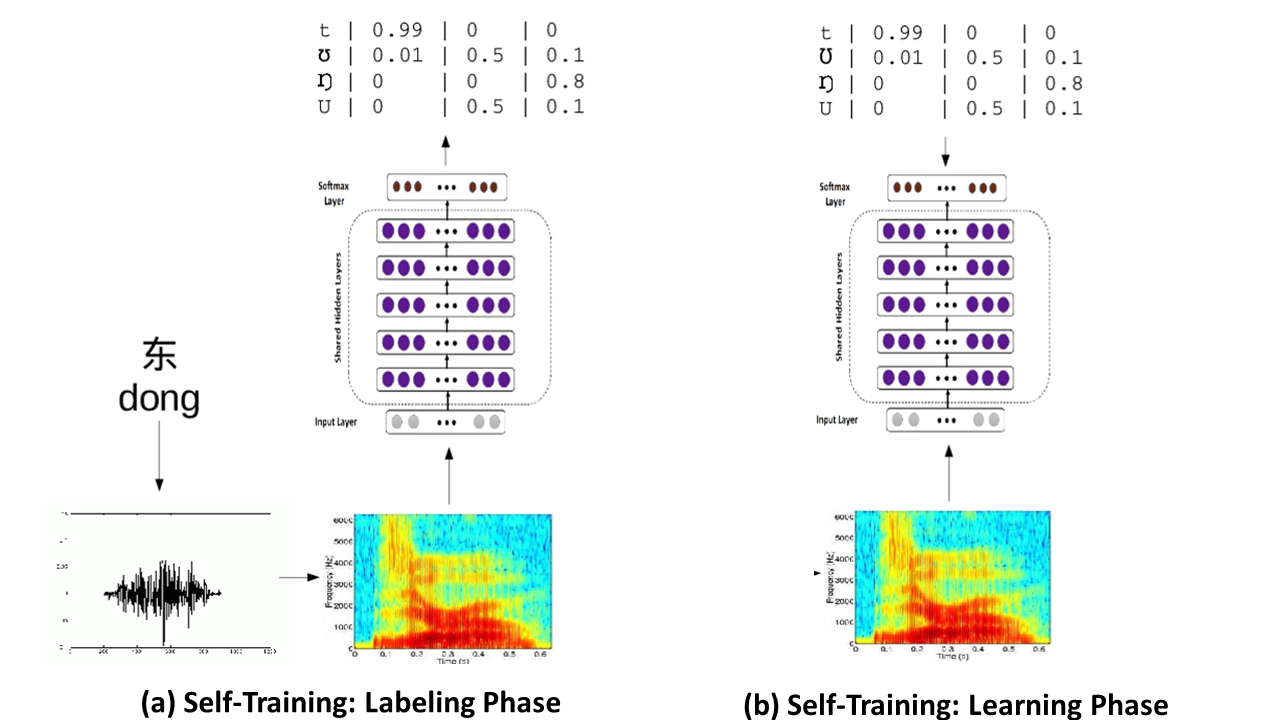
\includegraphics[width=5in]{../figs/fig_hager.png}}
%  \caption{The self-training method of~\cite{vesely2013-semi} includes
%    a labeling phase and a learning phase.  (a) Labeling phase: an ASR
%    trained on other languages (here Cantonese) is used to compute
%    posterior phone probabilities $\pi(\phi_t^\ell|x^\ell)$ in the
%    test language (here Mandarin). (b) Learning phase: posterior phone
%    probabilities are used as targets for NN re-training.}
%  \label{fig:hager}
%\end{figure}
%% comments: since the key difference in this figure between the
%% labeling phase and the learning phase is the direction of the upper
%% arrow, I suggest making the arrows more prominent. Also, the text
%% annotating the NN is illegible, as is the text garnishing the axes
%% of the waveform and spectrograms.
Experiments using other datasets found that the best self-training
uses best path alignment to specify a binary target for NN
training~\cite{vesely2013-semi}, but, apparently because of
differences in the adaptation set between our experiments and previous
work, we achieve better performance using real-valued targets
$0\le\rho(s_t^\ell|x_t^\ell)\le 1$.
%(Fig.~\ref{fig:hager}). However, we did follow the recommendation in
%\cite{vesely2013-semi} to scale the amount of transcribed data by 2 to 
%create a good balance between transcribed and untranscribed data.
